
%%%%%%%%%%%%%%%%%%%%%%%%%%%%%%%%%%%%%%%%%%%%%%
\section{Photon Detection System (PDS)}
\label{sec:pd_system}

LAr is an excellent scintillating medium and the photon detection
system (PDS) is used to obtain additional event information from
the photons produced by particles traversing the detector.
 With an
average energy of 19.5~eV needed to produce a photon (at zero field),
a typical particle depositing 1~MeV in LAr generates
40,000~photons with a wavelength of 128~nm. In higher electric fields this number is 
reduced, but at 500~V/cm the yield is still $\sim$20,000~photons
per MeV. Roughly 1/4 of the photons are promptly emitted with a
lifetime of about 6\,ns, while the rest are produced with a lifetime of
1100--1600~ns. Prompt and delayed photons are detected in
  precisely the same way by the photon detection system. LAr is
highly transparent to the 128-nm VUV photons with a Rayleigh
scattering length of (66~$\pm$~3)\,cm~\cite{Rayleigh} 
\fixme{Missing this citation in common/pdune-tdr-citedb.bib''}
and absorption
length of $>$200~cm; assuming a LN$_2$
  content of less than 20~ppm. The relatively large light output makes
the scintillation process an excellent candidate for determining the
$t_0$ for non-beam related events. Detection of the scintillation
light can also be helpful in performing background rejection and triggering on
non-beam events.

%%%%%%%%%%%%%%%%%%%%%%%%
\subsection{Scope and requirements}

The photon detector system (PDS) 
includes the following components:

\begin{itemize}
\item Light collection system including wavelength shifter and light guides
\item Light sensors: Silicon photo-multipliers (SiPMs)
\item Readout electronics
\item Monitoring system
\item Related infrastructure (frames, mounting boards, etc.).
\end{itemize}


The primary requirement is the detection of light from proton decay
candidates (as well as beam neutrino events) with high efficiency to
enable 3D spatial localization of candidate events. The assumed light yield necessary for
meeting this requirement is 0.1\,pe/MeV for a particle track near the cathode plane
(the farthest possible location from the PDS). In DUNE, 
the TPC  provides supernova neutrino detection, while the detection of light
from supernova neutrino interactions localize the events and disentangles
them from background noise in the TPC.
The photon system provides the $t_0$  of
events relative to TPC timing with a resolution better than 1~$\mu$s
(providing position resolution along the drift direction on the order of a couple of mm). 
Measurements %from the ProtoDUNE-SP detector 
will determine the absolute
light yield by measuring light from beam particles and cosmic ray muons
tracked in the TPC or identified by external muon trigger counters.

Figure~\ref{fig:PD_overview} shows the layout for the photon detector
system described in this section. %, which will be described in the following sections.

\begin{cdrfigure}[Photon detection system overview]{PD_overview}{Overview of the PDS
    system showing a cartoon schematic (a) of a single PDS module
    in the LAr and the channel ganging scheme used to reduce the
    number of readout channels. Panel (b) shows how each PDS module
   is inserted into an APA frame. Ten photon detectors (PDs) are inserted
    into an APA frame.}
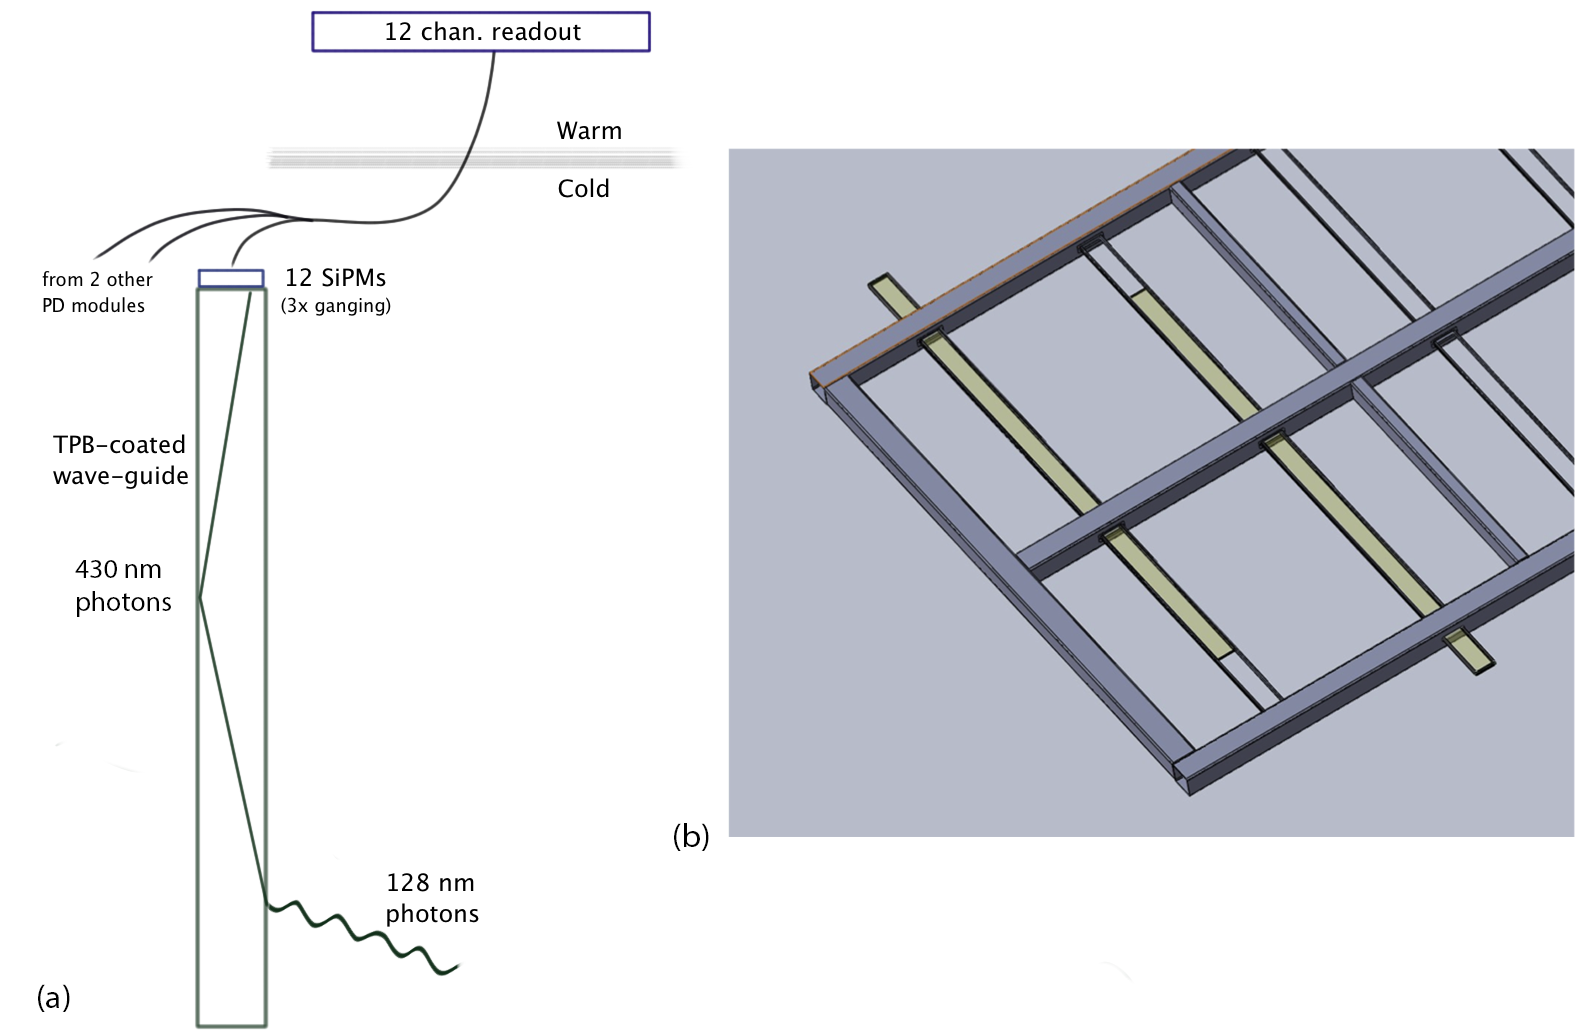
\includegraphics[width=1.0\linewidth]{pd_schem.png}
\end{cdrfigure}

%%%%%%%%%%%%%%%%%%%%%%%%%%
\subsection{Photon detector modules}

Two different styles of PDS 
modules are planned to be installed in the detector.  The two designs test similar light-collection strategies, which differ primarily in  the number of times the LAr scintillation 
light is shifted.  

The first design, shown schematically in Figure~\ref{fig:PD_overview}. is based on
wavelength-shifting radiator plates mounted to wavelength-shifting light guides.
The plates are coated 
with tetraphenyl-butadiene (TPB) to produce blue ($430nm$) light from the 128-nm VUV 
scintillation light.  
This blue light is absorbed by the commercially produced wavelength shifting (WLS)
polystyrene bar with Y-11 fluor, producing green light, which is transmitted
through the light guide to the photosensor 
mounted at its end.
The radiator plates are held captive in mounting blocks that are glued to the WLS bar
at regular intervals as shown in Figure~\ref{fig:PD_radiator_mount}.

\begin{cdrfigure}[Radiator Plate Mounting Blocks]{PD_radiator_mount}
  {Mounting of the radiator plates to the WLS bar for the reference design scheme}
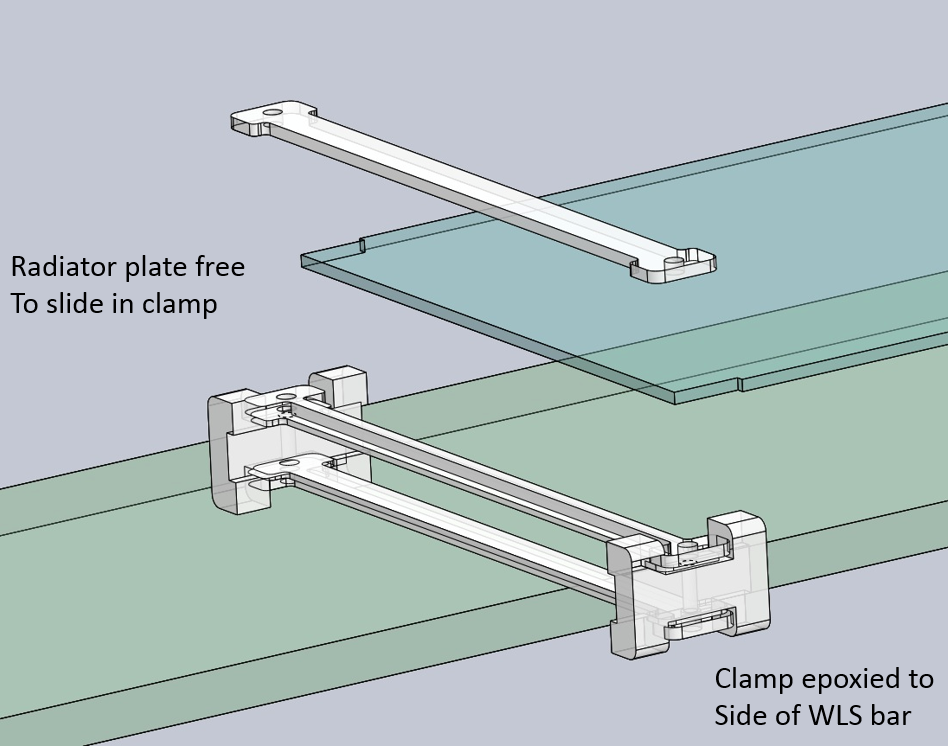
\includegraphics[width=0.5\linewidth]{PD_radiator_mount.PNG}
\end{cdrfigure}

The second design uses the same mounting, but with no radiator plates installed.  
Instead, an acrylic light-guide bar is dip-coated  with a solution
of TPB, solvents, and a surfactant to produce a wavelength-shifting layer on the
outside surface of the bar.
The 128-nm VUV scintillation light is shifted directly tio \fixme{?} and transmitted
through the lightguide to the photosensor. Because the design uses only one wavelength shifting step, potential efficiency increases are possible.


%%%%%%%%%%%%%%%%%%%%%%%%%%
\subsection{Sensors}

The planned photodetector is a SiPM, model 
SensL C-Series 6~mm$^2$
(MicroFB-60035-SMT). % device. 
This model of SiPM has a detection efficiency of
41\%; the quoted detection efficiency incorporates Quantum Efficiency (QE) and 
the effective area
  coverage accounting for dead space between pixels.   At LAr temperature (89~K) the dark rate is of order 10~Hz
(0.5 p.e. threshold), and  after-pulsing has not been observed. An on-going testing program is in place to ensure 
that the SiPMs can reliably survive the stresses associated with 
any thermal cycling in LAr and long-term operation at LAr temperature.

All photodetectors %for ProtoDUNE-SP 
are subjected to testing to determine
 forward and reverse bias I-V curves,
 breakdown voltage, dark current and dark count rate, photodetector gain, crosstalk estimation, response, and bias dependence of parameters.
 
%All SiPMs 
Each SiPM is tested before mounting on the readout boards to determine
if the part meets the specifications in a warm test.  After mounting to
the readout board all items are tested both warm and cold (cyrogenic 
temperature) to determine the operating characteristics.

In addition to these tests, the photodetectors are tested for their
response to light signals from an LED of appropriate wavelength.
These tests will be sensitive enough to determine if one of the three SiPM
elements operating in parallel is not functioning.


%%%%%%%%%%%%%%%%%%%%%%%%%%
\subsection{Mechanical design and installation}
  % -- CSU  -- Dave
  %  Mechanical Design Mounting 

The PDS is configured as a set of \textit{modules} that are mounted on the APA frames.  A PDS module is
the combination of one light guide (also called a ``bar'' due to its
shape) and 12 SiPMs, as shown in Figure~\ref{fig:PD_overview}~(a). 
The APA frames hold ten PDS modules, approximately 2.2-m long,
86-mm wide and 6-mm thick, equally spaced along the full length of the
APA frame, as shown in Figure~\ref{fig:PD_overview}~(b). 
The light guides are inserted into the APA frame on rails gliding on their radiator
plate mounting blocks, as shown in Figure~\ref{fig:PD_mounting_inslide} (right). \fixme{check if right figure ref}

\begin{cdrfigure}[Diagram of PDS installation into APA frame and installed SiPM mounting board]
  {PD_mounting_inslide}{(left) Rendering of the installation of a PDS module
    into an APA frame, shown just before it comes to rest on the inside face
    of the APA tube. (right) Rendering of the the SiPM mounting board
    installed on the end of the PDS module before insertion.}
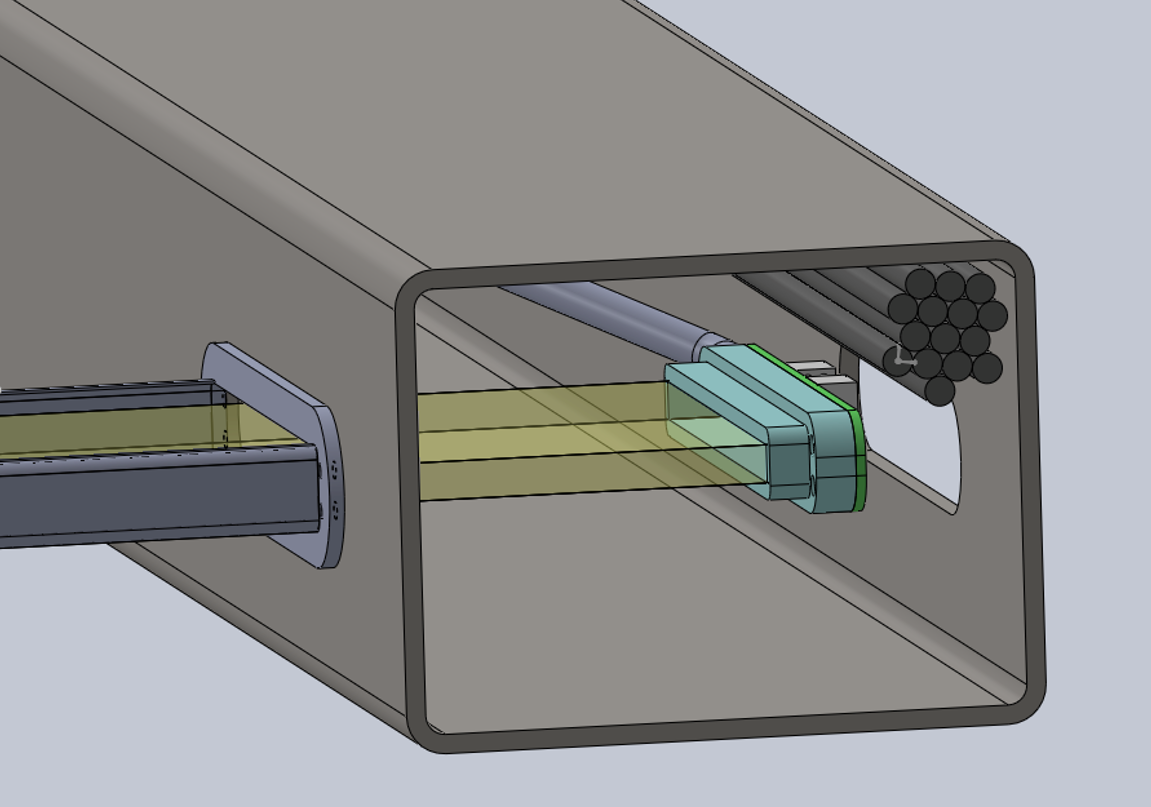
\includegraphics[width=0.456\linewidth]{PD_mounting_inslide.PNG}
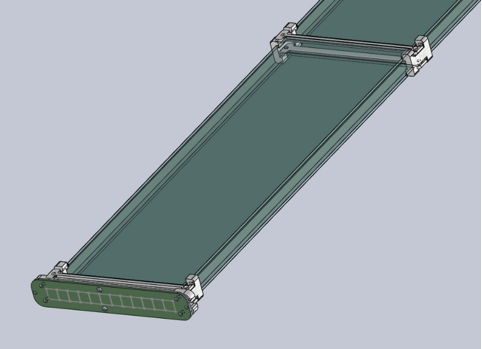
\includegraphics[width=0.444\linewidth]{PD_endblock_mnt.PNG}
\end{cdrfigure}

The mounting system has been tested using a prototype PDS module  
as shown in Figure~\ref{fig:PD_flat_installtest}.
\begin{cdrfigure}[Photo of PD mock installation]
  {PD_flat_installtest}{Photograph of the installation
    test of a mock PDS module in a 1/5 section of an APA frame.}
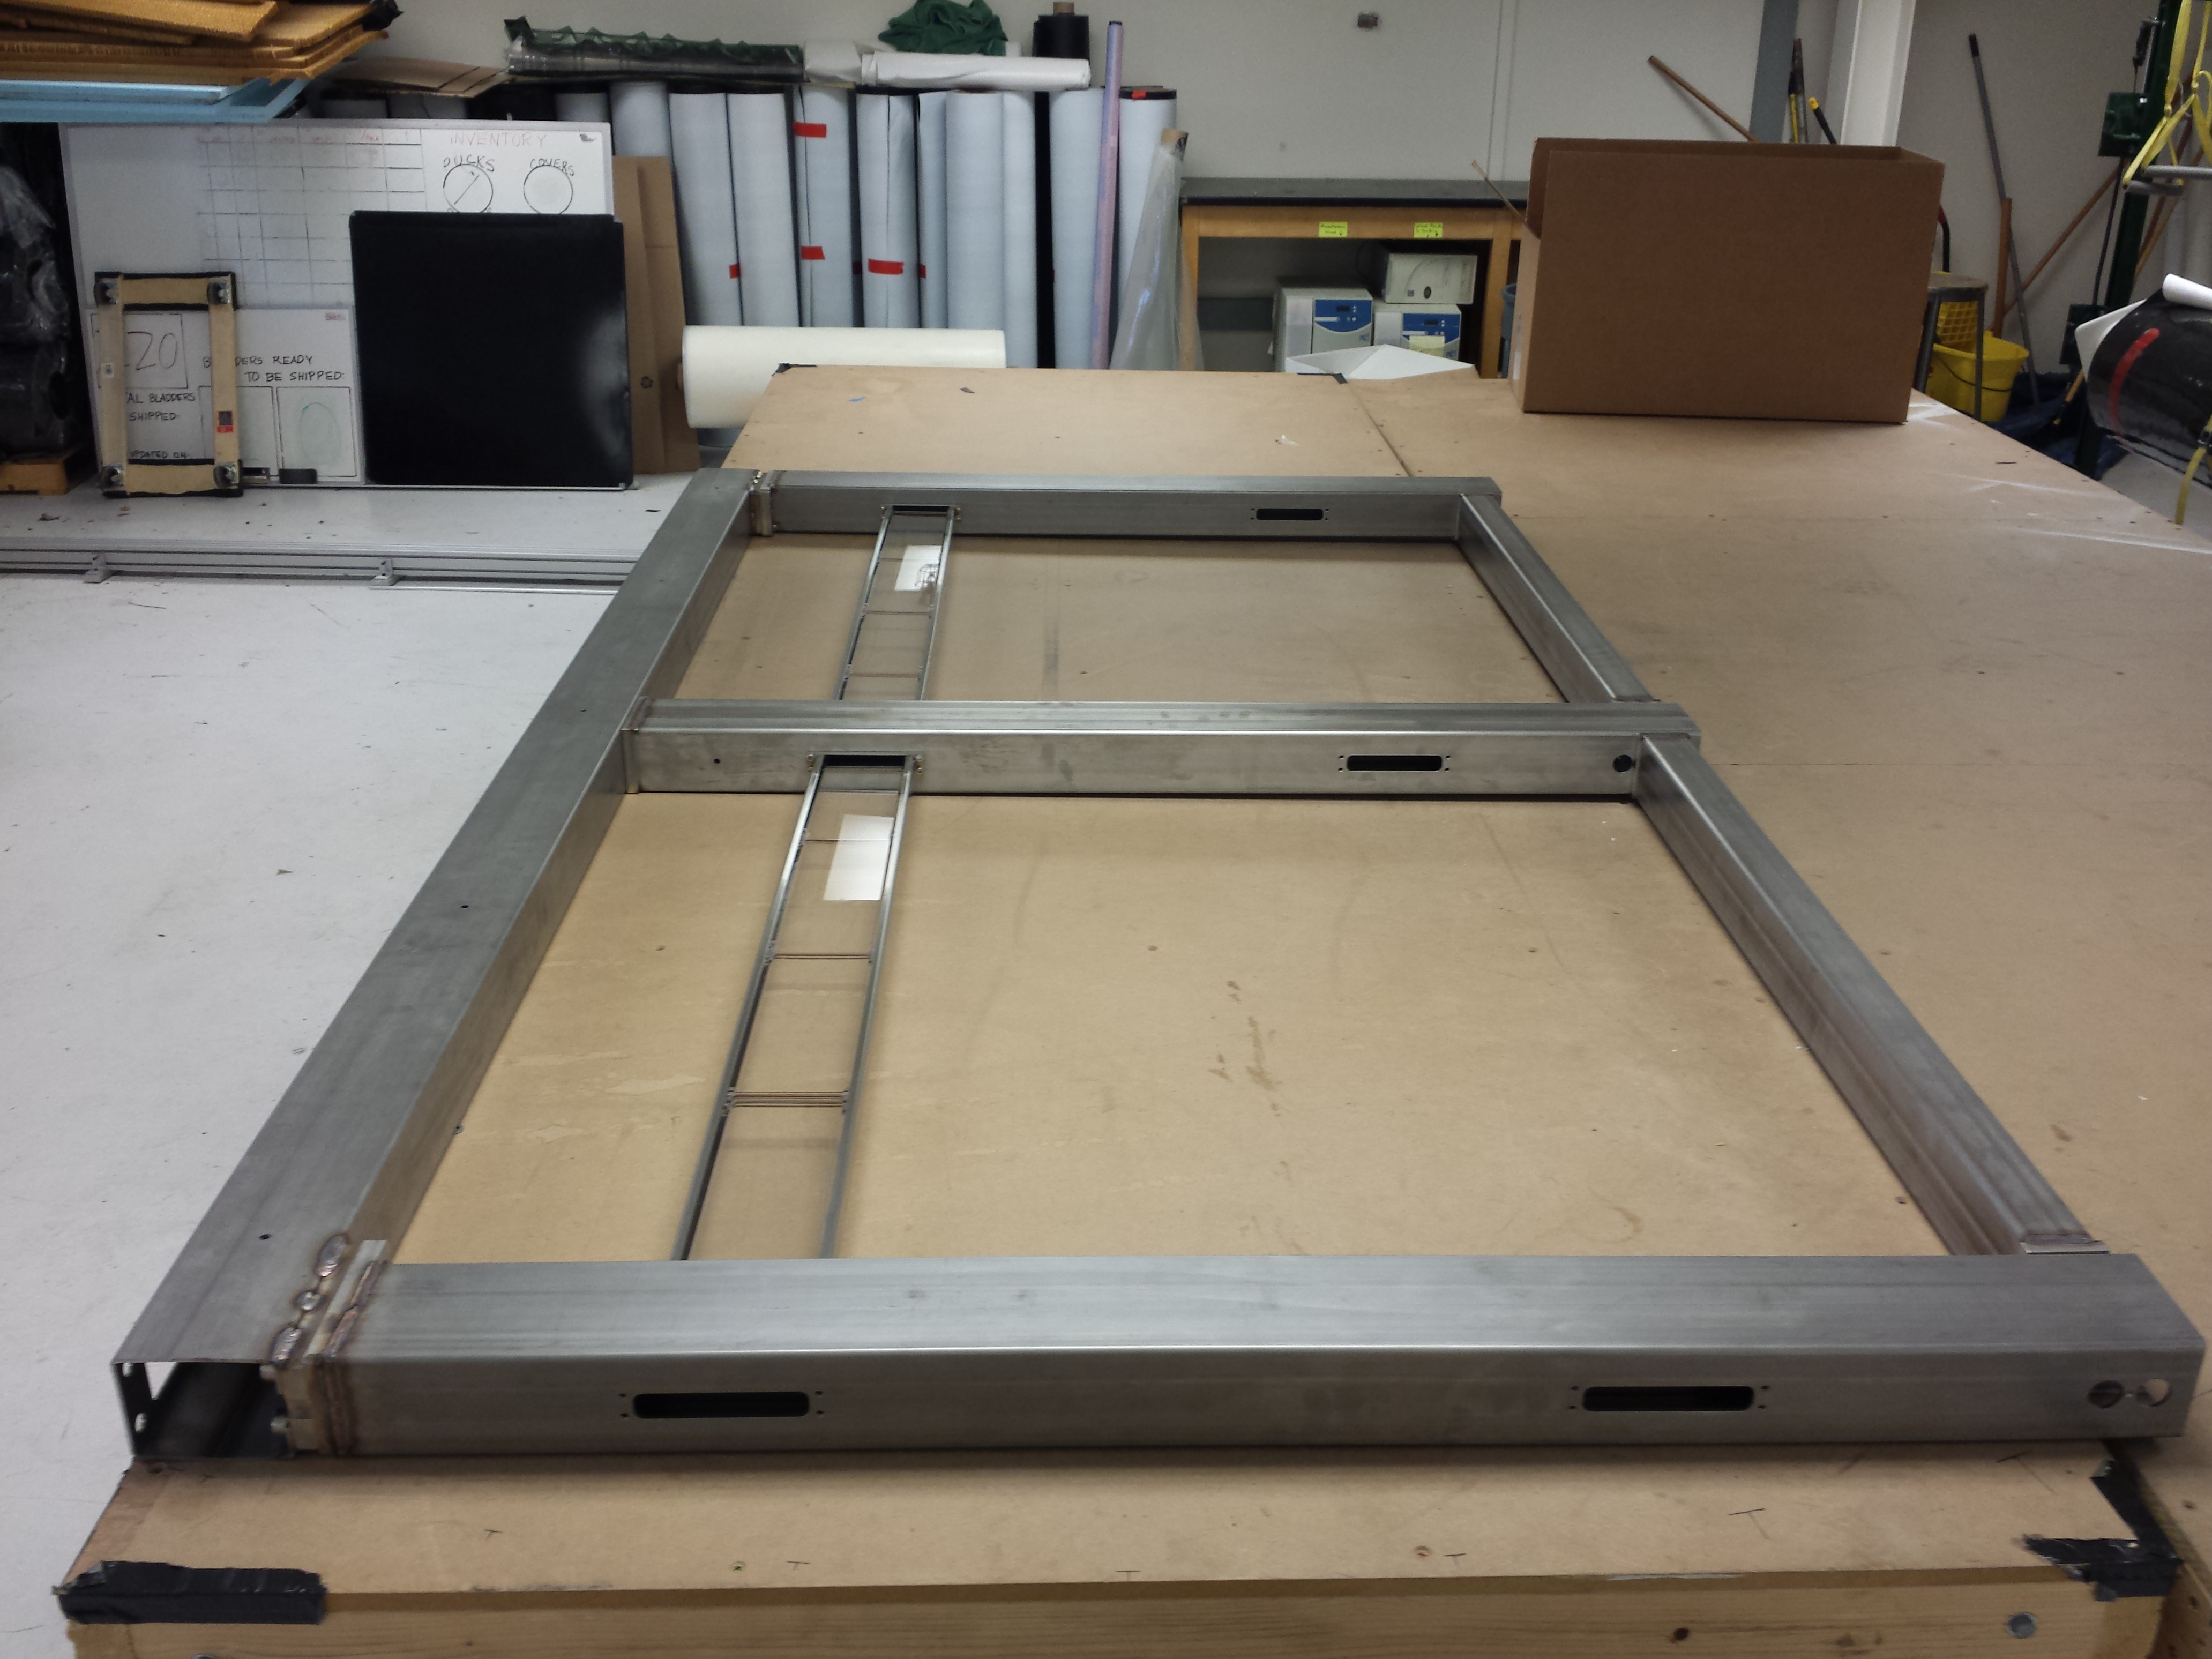
\includegraphics[width=0.50\linewidth]{pd_flat_installtest.jpg}
\end{cdrfigure}


Each photon detector has a single SiPM mounting board with 12 surface-mount SiPMs 
mounted on its face as shown in Figure~\ref{fig:PD_SiPM_PCB_front} (left).
Four groups of $3$ SiPM elements go to single 
channels of the readout electronics in order to reduce the overall system cost.
The board is held close to the bar, without touching, using four screws that go into 
tapped holes on the end mounting block that is glued to the bar.  
The mounting block assembly is shown in Figure~\ref{fig:PD_mounting_inslide} (right) %\ref{fig:PD_endblock_mnt}.
The circuit board also has holes at each end for mounting to the APA frame.  

\begin{cdrfigure}[SiPM mounting board with 12 SiPMs and with Rj-45 connector]
  {PD_SiPM_PCB_front}{Photograph of a SiPM mounting board
    with the full complement of 12 SiPMs installed on the board (left), and with the 
    RJ-45 connector for the cable (right).}
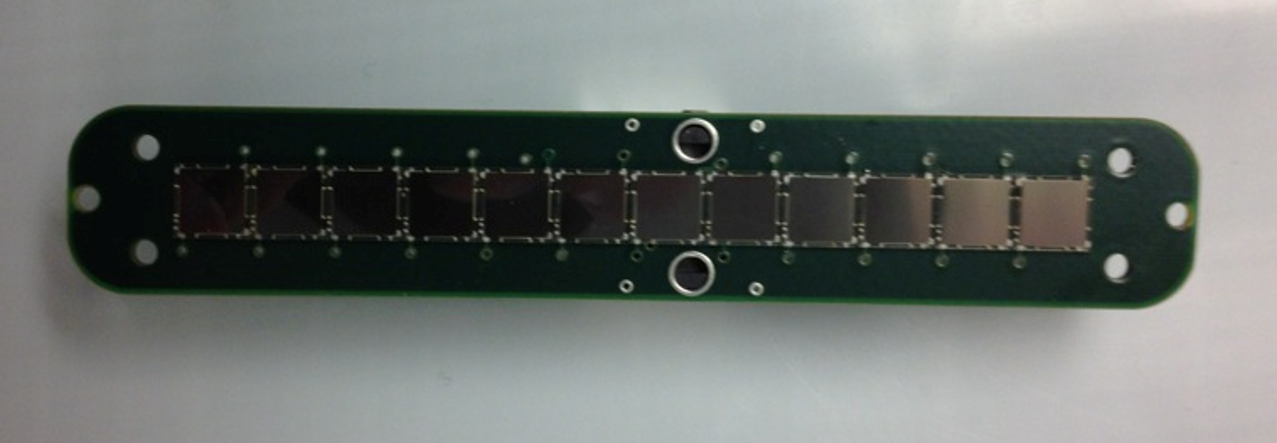
\includegraphics[width=0.55\linewidth]{PD_SiPMMountPCB_front.PNG}
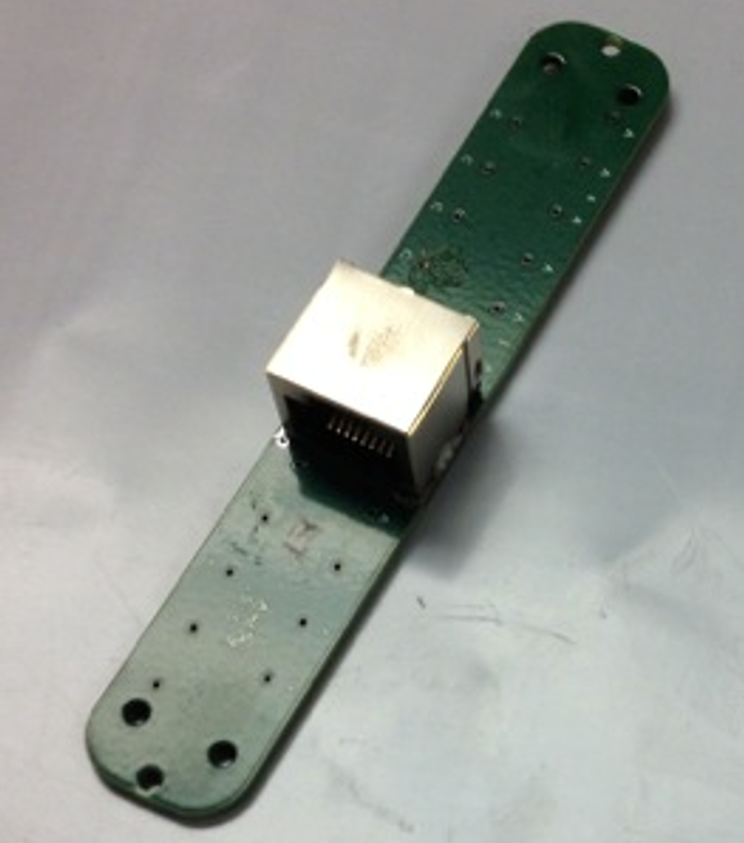
\includegraphics[width=0.4\linewidth]{PD_SiPMMountPCB_back.PNG}
\end{cdrfigure}
%\begin{cdrfigure}[Readout board with RJ-45 connector]
%  {PD_SiPMMountPCB_back}{Photograph of the SiPM readout PCB with the 
%    RJ-45 connector for the cable.}
%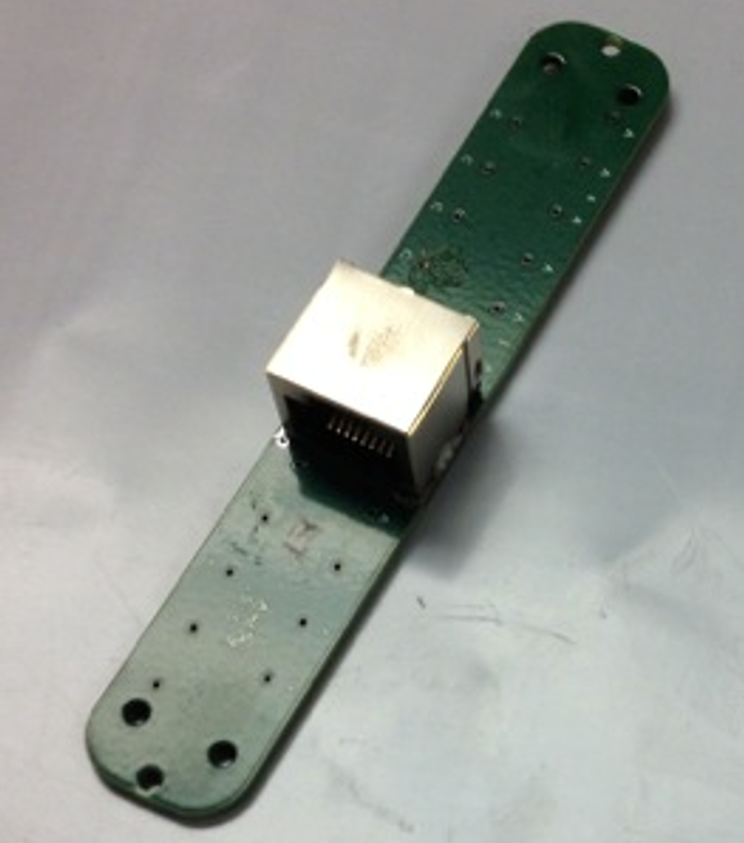
\includegraphics[width=0.50\linewidth]{PD_SiPMMountPCB_back.PNG}
%\end{cdrfigure}

  %   Mechanical Design Cabling

The cabling plan for the system has one cable with four shielded twisted pairs 
connected to each SiPM mounting board via the surface mount RJ-45 connector
shown mounted on the back of the readout PCB in 
Figure~\ref{fig:PD_SiPM_PCB_front} (right).  
The cables run through the APA tubing to the top of the APA frame as seen
in Figure~\ref{fig:PD_cable_intube}.
The cable bundles are installed and connected 
after the PD has been installed into the slot.
\begin{cdrfigure}[Cables in APA frame]
  {PD_cable_intube}{Diagram showing the routing of the PDS cables
    through the APA frame.}
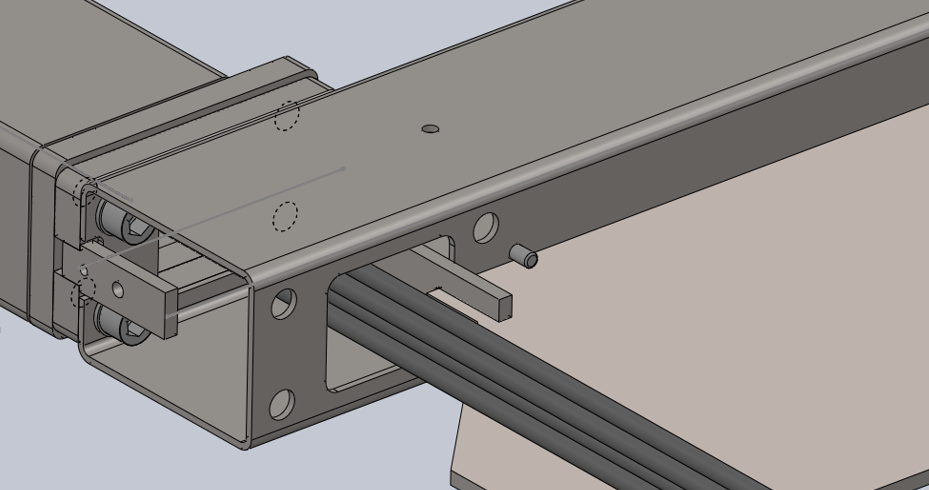
\includegraphics[width=0.50\linewidth]{PD_cable_intube.PNG}
\end{cdrfigure}


%%%%%%%%%%%%%%%%%%%%%%%%%%
\subsection{Alternative photo detector under development}

While a sufficient number of the two types of PDS modules are being produced to fully outfit the detector, it is possible that a few of the 60 APA slots will be used to house experimental photon detectors. One type of detector that is being developed in an attempt to increase the light detection eficiency is referred to as the ARAPUCA design.

The ARAPUCA design is based on a new technology that allows for the collection of photons in a 5$\times$5-cm$^2$ window  with detection efficiencies at the level of several percent. The trapped light is detected by two SIPMs (SensL 60035 - 6$\times$6 mm$^2$ active area each). The basic concept behind the ARAPUCA design is to trap photons inside a teflon box, of  dimensions of 5$\times$5$\times$1 cm$^3$, with highly reflective internal surfaces, such that the detection efficiency of the trapped photons remains high even with limited sensor coverage on these internal surfaces~\cite{Machado:2016jqe}.

Photon trapping is achieved by using a wavelength-shifting technique coupled with the technology of the dichroic shortpass optical filters. The latter are multilayer acrylic films 
with the  property of being highly transparent to photons with a wavelength below a tunable cut-off while being almost perfectly reflective to photons with wavelength above the cut-off. 
A dichroic shortpass filter deposited with two different wavelength shifters (one on each side) is the core of the device. In particular, it serves as the acceptance window for the 
ARAPUCA device. The rest of the device is a flattened box with highly reflective internal surfaces (PTFE, 3M-VIKUITI ESR, \dots), closed on the top by the 
dichroic  filter deposited with the two shifters. A fraction of the internal surface of the box is occupied by the active photo-sensors (Silicon Photomultipliers, or SiPMs) that detect the trapped photons.

It is envisioned that several of these devices could be installed on the detecotr to directly compare their performances with those of the
other PDS modules. A mechanical solution has been developed such that 16 of the ARAPUCA devices can be installed on the same mounting structure used for the other PDS modules as shown in Figure~\ref{fig:arapuca_array}.
%*****************************FIGURE 2*****************************%
\begin{cdrfigure}[ARAPUCA array installed in a APA frame]
  {arapuca_array}{One ARAPUCA array of eight devices installed in a APA frame in place of a scintillating bar.}
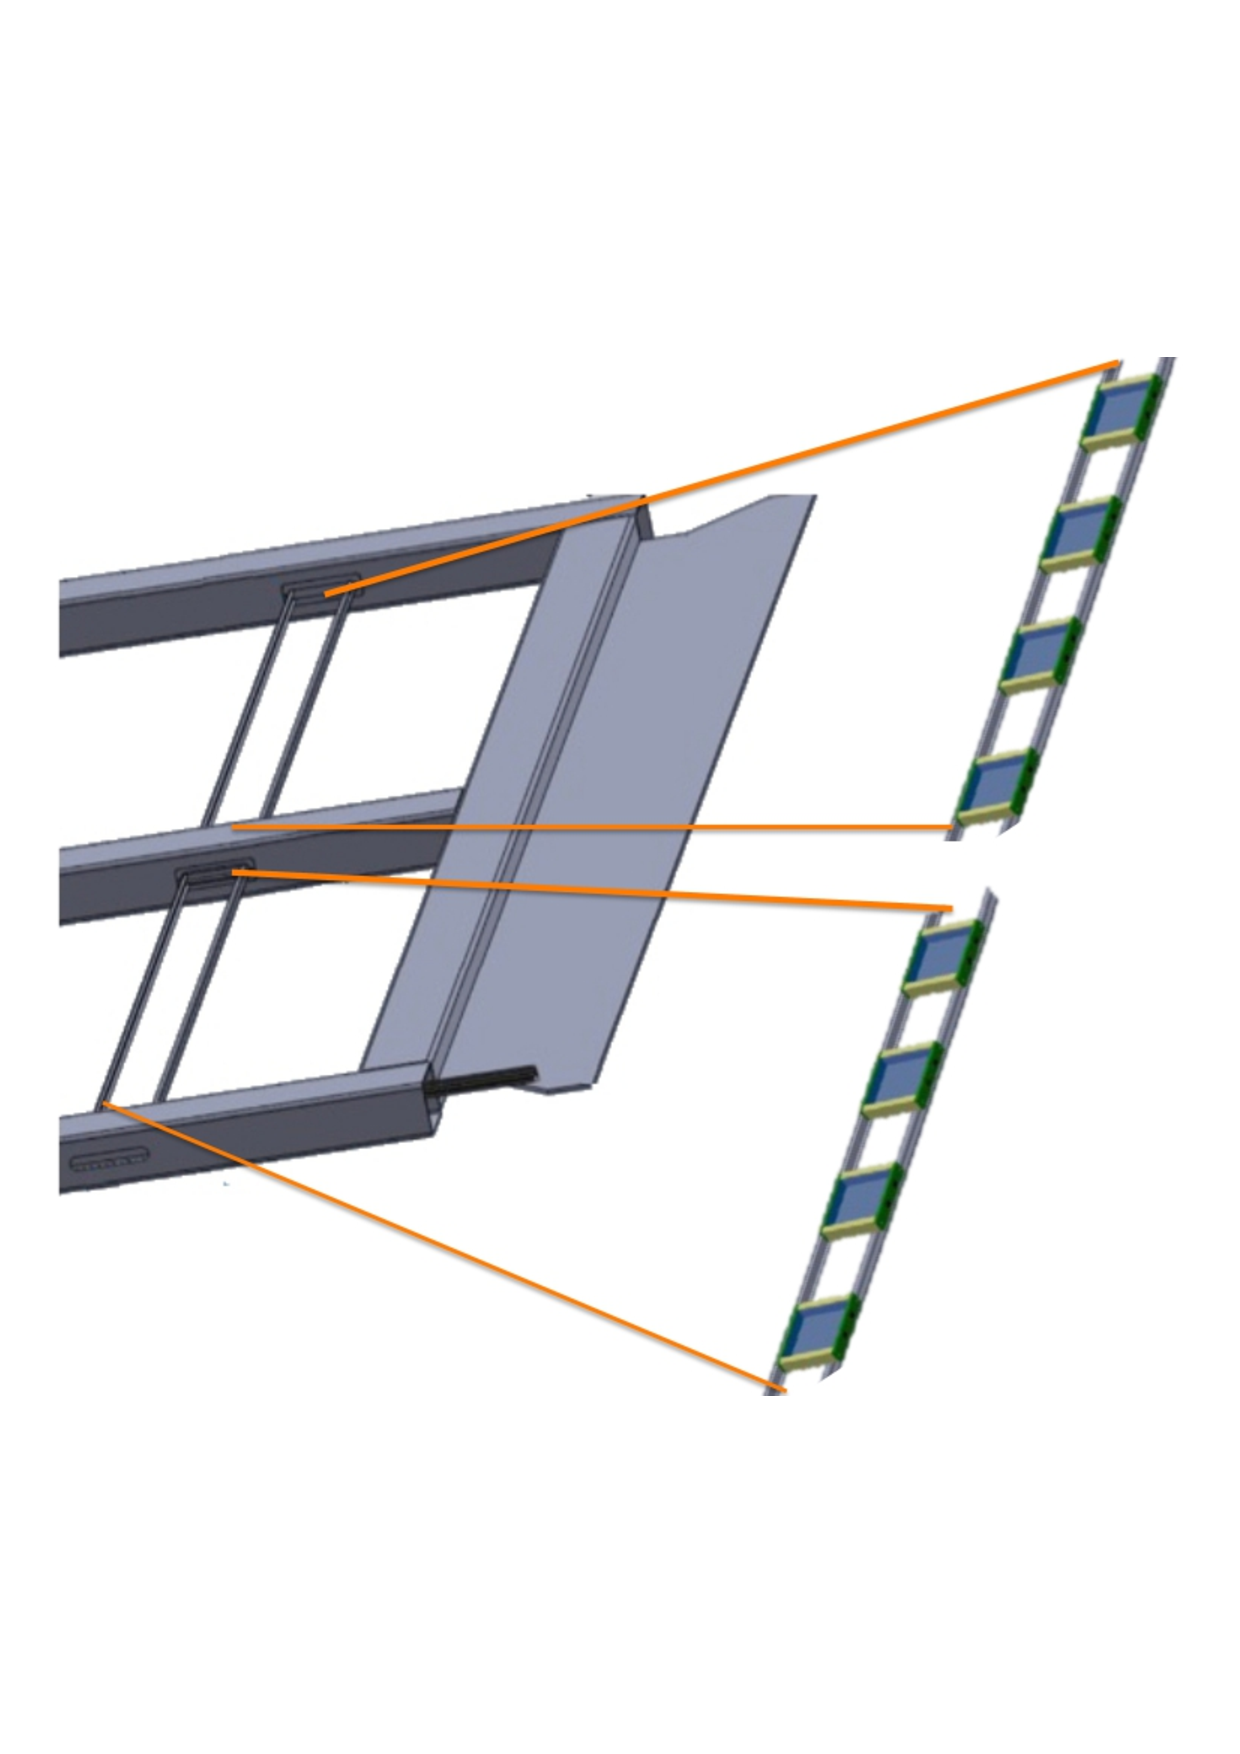
\includegraphics[width=0.50\linewidth]{APA_ARAPUCA}
\end{cdrfigure}

%***********************************************************************%
The readout scheme foresees the ganging of the SiPMs from two ARAPUCA devices (four sensors total). The 16 devices on one mounting structure then have a total of four readout channels, which can take advantage of the same cabling and readout scheme used for the other PDS modules.

%%%%%%%%%%%%%%%%%%%%%%%%%%
\subsection{Photon detector UV-light monitoring system}
\label{sec_pd_calib}

A UV-light-based monitoring system is used to monitor the relative performance and time resolution of the system.
The system uses external UV LEDs (245-280\,nm) as light sources in the VUV wavelength range, which are coupled to quartz fibers to transmit light from outside the detector volume to desired locations on the CPA plane.
Light diffusers located on the CPA surface uniformly illuminate the APA area 
containing the  PDS.
The UV light system is used in association with cosmic ray muon 
tracks and Michel electrons as means of calibration.
The UV light essentially mimics physics, although at a different wavelength starting from the wavelength-shifter conversion, 
light guide propagation, photo-sensor detection and the front-end electronics readout.
	
The external UV-light monitoring system is designed with the following goals:
				
\begin{itemize}
\item No active components within PD/APA;
\item Provide uniform illumination over the APA surfaces;
\end{itemize}

In terms of technical requirements the system needs to:
\begin{itemize}
\item provide light levels down to a single p.e. for individual photon-detector channels,
\item provide higher light levels to test linearity of the PDS,
\item provide variable pulse width to test the time resolution of the photon detector response, and
\end{itemize}

Figure~\ref{fig:fig-c-1} illustrates the system design schematically. The system consists of a 1U rack mount Light Calibration Module (LCM) sitting outside the cryostat. The LCM generates light pulses that propagate through a quartz fiber-optic cable to diffusers at the CPA to distribute the light uniformly across the photon detectors mounted within the APA.  Five light 
diffusers on the CPA plane are used: one in the center and four diffusers close to the CPA corners. 
%
 \begin{cdrfigure}[UV-light monitoring system]{fig-c-1}{Concept of the UV-light monitoring system for the photon detector in liquid argon.}
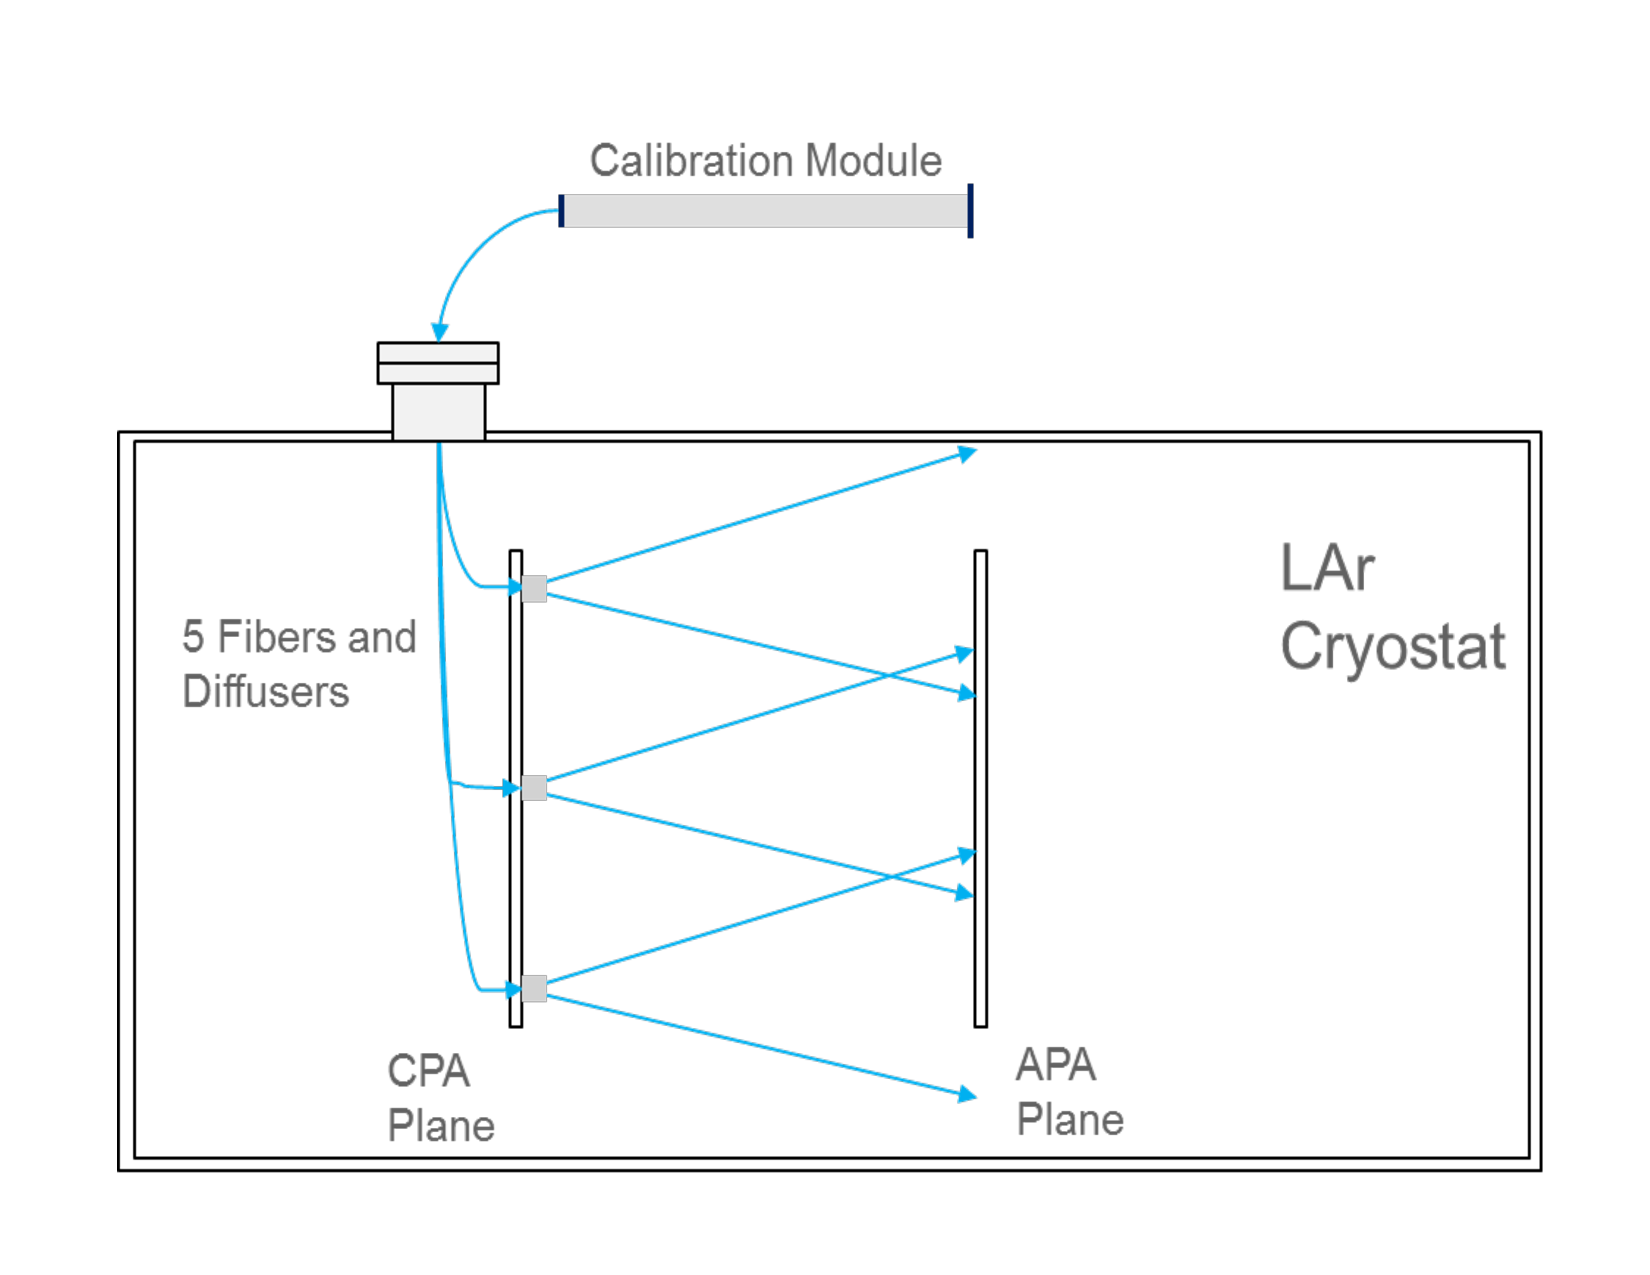
\includegraphics[angle=0,width=0.7\textwidth]{calPD_concept-from-35ton.pdf}
\end{cdrfigure}
%


The LCM utilizes the logic and timing control of the photon-detector readout electronics (\textit{SSP}) unit, described in Section~\ref{sec:pds-elec-daq}.  
A single SSP board was repackaged into a deeper rack mount chassis that accommodates a new internal 
LED Pulser Module (LPM) and an additional bulk power supply. The LPM utilizes five digital outputs from the SSP board to control the LPM pulse and its duration.  
These outputs are derived from the charge injection control logic within the SSP's FPGA.  
The even-channel SiPM bias Digital to Analog Converters (DACs)
are used to control the LPM pulse amplitude.  
The adjacent odd channels are used to read out a reference photodiode used for pulse-by-pulse monitoring of the LED light output.  
The output of the monitoring diode is available for normalizing 
the response of the SiPMs in the detector to the monitoring pulse.


\fixme{A bunch of content removed from here; but then gap in (paper) pages received from Flavio (missing 4-147 to 4-180); not sure what to do with remainder of this file. Anne}

\fixme{How long do these monitoring run take ? When would they be taken (relative to beam and comics running) ? Some interference with light from comics is expected; how will this be addressed ? Time of a flash will be known much better then 1us, so not much overlap with random cosmic events at ~1ms }

The controlled source of light  
in this monitoring system is used to perform time offset and time resolution measurements.  
Many effects contribute to a finite time resolution, including the relative time offset of photon-detector channels, scintillation time constants, 
photon conversion with wavelength shifter, photon propagation through photon-detector paddle, SiPM jitter, and FEE resolution. \fixme{FEE = front end electronics?}
Most of these effects are constant and can be individually 
measured on the bench.  The UV light monitoring system monitors overall stability of the photon detector in both time
and amplitude.
